%**************************************************************
% Lab 10: RAM
%**************************************************************
\chapter{RAM}

\section{Purpose}

This lab is used to demonstrate how a \acf{RAM} device operates. 

\section{Procedure}

A RAM (\textit{Memory} library) device is similar to a ROM device as used in Lab \ref{Lab09}, \nameref{Lab09}. A RAM device has an address input port, a data port, and several control ports. An address is loaded in the Address Port then on the next clock signal the device either reads the data at that address and outputs it on the data port or inputs whatever is on the data port and writes it to that address. Figure \ref{fig:10-01} illustrates a counter connected to a RAM address port so as the counter outputs an increasing value the RAM will ``step through'' memory locations.

\begin{figure}[H]
	\centering
	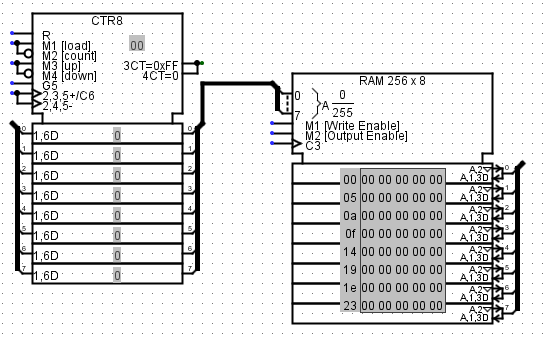
\includegraphics[width=\maxwidth{.95\linewidth}]{gfx/10-01}
	\caption{RAM Basics}
	\label{fig:10-01}
\end{figure}

In operation, a high signal on RAM port M1 enables the write function and the RAM device will store whatever is present on the data ports into the address pointed to on the address port. A high signal on port M2 enables the output function (a ``read'' function) and the RAM device will send whatever is present in the address pointed to on the address port to the data ports.

Notice that the data ports have both an in and out pointing arrow to indicate that those ports are designed for both input and output, depending on the setting of M1 and M2.

Figure \ref{fig:10-02} shows a RAM device with the various control signals. (Note: to show more detail, the right edge of the RAM device was cut from the figure.)

\begin{figure}[H]
	\centering
	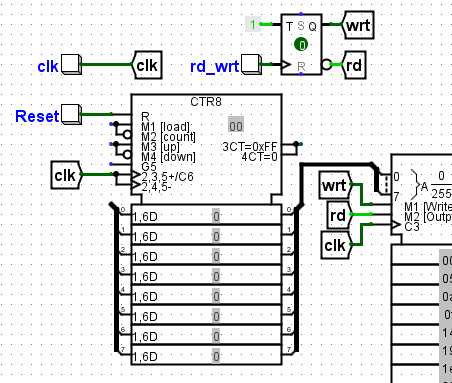
\includegraphics[width=\maxwidth{.95\linewidth}]{gfx/10-02}
	\caption{RAM With Control Signals}
	\label{fig:10-02}
\end{figure}

\marginpar{To simplify the circuit wiring, tunnels are used to transport various signals around the circuit.}At the top left of the subcircuit a button is used to generate a clock pulse. By using a button students can pulse the circuit slowly and observe how the RAM device operates. In an actual circuit that button would be replaced by a Clock (\textit{Wiring} library).

At the top of the circuit is a T Flip-Flop (\textit{Memory} library) that is used to control whether the RAM device is reading or writing data. Because it is important that M1 and M2, the two control ports on the RAM device, are never both high at one time a flip-flop is the perfect controller. The T input on the flip-flop is tied to a constant high so whenever the rd\_wrt button is pressed the RAM device toggles between read and write functions.

The Counter has a Reset button attached that will reset its count to zero so the RAM device will always either read or write from its lowest memory location. In actual practice the counter would need a much more complex circuit to set a specific start point for the RAM device to read or write but for this simple demonstration circuit it is enough to always start read/write operations from the lowest memory location.

The next step is to set up the data bus on the east side of the RAM device. It is important that the bus does not attempt to carry data out of the RAM device at the same time that data are being sent to the RAM device. Thus, control buffers are used to determine the direction of data flow between the RAM device and the data bus. Figure \ref{fig:10-03} shows the data bus with the control buffers. (Note: to show more detail, the counter was cut from the left edge of the figure.)

\begin{figure}[H]
	\centering
	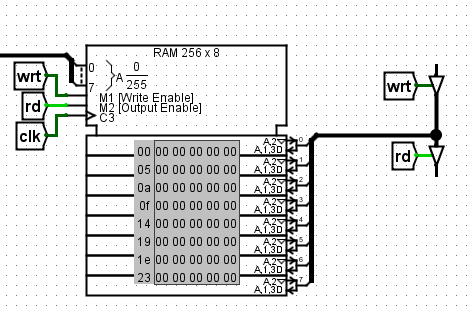
\includegraphics[width=\maxwidth{.95\linewidth}]{gfx/10-03}
	\caption{Data Bus}
	\label{fig:10-03}
\end{figure}

Notice that the outputs of the read/write flip-flop are being used to control the direction of the data flow for the RAM device.

To complete the demonstration circuit, a Keyboard (\textit{Input/Output} library) device is added to write ASCII characters into RAM memory and a TTY (\textit{Input/Output} library) device is used to display ASCII characters read from RAM memory. Figure \ref{fig:10-04} shows the input/output devices. (Note: to show more detail, part of the RAM and TTY devices were cut from the edges of the figure.)

\begin{figure}[H]
	\centering
	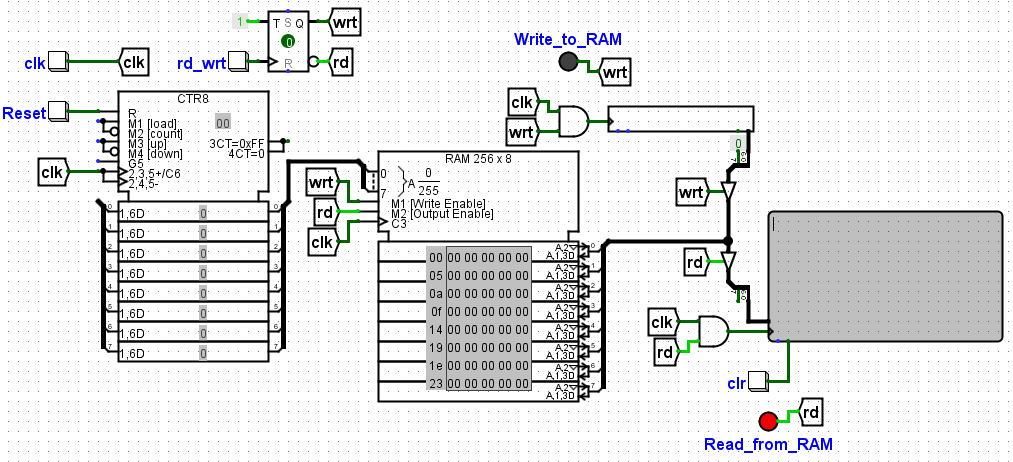
\includegraphics[width=\maxwidth{.95\linewidth}]{gfx/10-04}
	\caption{RAM With Input/Output Devices}
	\label{fig:10-04}
\end{figure}

For reference, the entire circuit is in Figure \ref{fig:10-05}.

\begin{figure}[H]
	\centering
	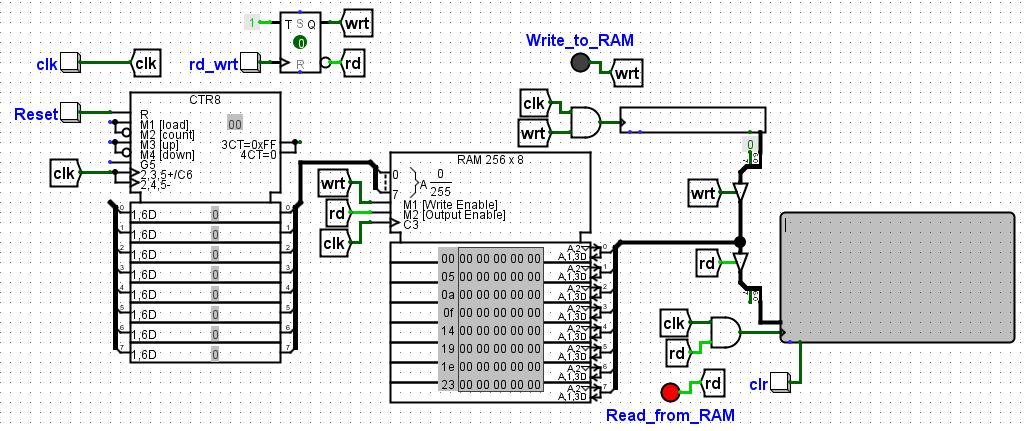
\includegraphics[width=\maxwidth{.95\linewidth}]{gfx/10-05}
	\caption{RAM With Input/Output Devices}
	\label{fig:10-05}
\end{figure}

To operate the keyboard device, click it and enter some text from the computer's keyboard. Then as that device is clocked one ASCII character at a time will be sent to the output port at its south-east corner. As in ASCII devices used in earlier labs, a splitter is used for both the keyboard and TTY display to strip the most significant bit from the data bus since the bus is eight bits wide but ASCII is only a seven-bit code.

Finally, two indicator LEDS have been added to make it clear whether data are being written to RAM or read from RAM.

\subsection{Testing the Circuit}

To test the complete circuit:

\begin{enumerate}
	\item Click Reset to set the counter to zero.
	\item Click the ``rd\_wrt'' button until the ``Write\_to\_RAM'' LED is on.
	\item Click the keyboard device and enter some text.
	\item Click the ``clk'' button to stream the text from the keyboard into RAM. Notice how the RAM device display changes to indicate the ASCII codes that have been stored.
	\item Click Reset to set the counter to zero.
	\item Click the ``clr'' button on the TTY device to clear that display.
	\item Click the ``rd\_wrt'' button until the ``Read\_from\_RAM'' LED is on.
	\item Click the ``clk'' button to stream text from RAM to the TTY device. Notice that this does not remove the text from RAM so it is still available for another reading if desired.
\end{enumerate}

\section{Challenge}

Build the circuit as described in this Lab and ensure that it operates as expected.

\section{Deliverable}

To receive a grade for this lab, complete the Challenge. Be sure the standard identifying information is at the top left of the \lstinline{main} circuit, similar to: 

\bigskip
% The minipage environment keeps the three lines together - no page break.
\begin{minipage}{\linewidth}
	\begin{verbatim}
	George Self
	Lab 10: RAM
	February 16, 2018
	\end{verbatim}
\end{minipage}
\bigskip

Save the file with this name: \textit{Lab10\_RAM} and submit that file for grading.
